% !TeX encoding = ISO-8859-1
%---------------------------------------------------------------------------
\documentclass[
    a4paper,                % paper format
    10pt,                   % fontsize
    oneside,                % double-sided
    openright,              % begin new chapter on right side
    notitlepage,            % use no standard title page
    parskip=half,           % set paragraph skip to half of a line
]{scrreprt}                 % KOMA-script report
%---------------------------------------------------------------------------

\raggedbottom
\KOMAoptions{cleardoublepage=plain}                     % Add header and footer on blank pages



% Load Standard Packages:
%---------------------------------------------------------------------------
\usepackage[standard-baselineskips]{cmbright}
\usepackage[ngerman]{babel}                             % german hyphenation
%\usepackage[ansinew]{inputenc}                         % Windows - load extended character set (ISO 8859-1)
\usepackage[latin1]{inputenc}                           % Linux - load extended character set (ISO 8859-1)
\usepackage[T1]{fontenc}                                % hyphenation of words with ���
\usepackage{textcomp}                                   % additional symbols
\usepackage{ae}                                         % better resolution of Type1-Fonts
\usepackage{fancyhdr}                                   % simple manipulation of header and footer
\usepackage{etoolbox}                                   % color manipulation of header and footer
\usepackage{graphicx}                                   % integration of images
\usepackage{float}                                      % floating objects
\usepackage{caption}                                    % for captions of figureMain documents and tables
\usepackage{booktabs}                                   % package for nicer tables
\usepackage{tocvsec2}                                   % provides means of controlling the sectional numbering
\usepackage[]{acronym}
\usepackage[acronym,toc]{glossaries}

%\usepackage[style=ieee,backend=biber]{biblatex}         %Bibliography
%\addbibresource{bibliography.bib}
%---------------------------------------------------------------------------

% Load Math Packages
%---------------------------------------------------------------------------
\usepackage{amsmath}                                    % various features to facilitate writing math formulas
\usepackage{amsthm}                                     % enhanced version of latex's newtheorem
\usepackage{amsfonts}                                   % set of miscellaneous TeX fonts that augment the standard CM
\usepackage{amssymb}                                    % mathematical special characters
\usepackage{exscale}                                    % mathematical size corresponds to textsize
%---------------------------------------------------------------------------

% Package to facilitate placement of boxes at absolute positions
%---------------------------------------------------------------------------
\usepackage[absolute]{textpos}
\setlength{\TPHorizModule}{1mm}
\setlength{\TPVertModule}{1mm}
%---------------------------------------------------------------------------
            
% Definition of Colors
%---------------------------------------------------------------------------
\RequirePackage{color}                                  % Color (not xcolor!)
\definecolor{linkblue}{rgb}{0,0,0.8}                    % Standard
\definecolor{darkblue}{rgb}{0,0.08,0.45}                % Dark blue
\definecolor{bfhgrey}{rgb}{0.41,0.49,0.57}              % BFH grey
%\definecolor{linkcolor}{rgb}{0,0,0.8}                  % Blue for the web- and cd-version!
\definecolor{linkcolor}{rgb}{0,0,0}                     % Black for the print-version!
%---------------------------------------------------------------------------

% Hyperref Package (Create links in a pdf)
%---------------------------------------------------------------------------
\usepackage[
    pdftex,ngerman,bookmarks,plainpages=false,pdfpagelabels,
    backref = {false},                                  % No index backreference
    colorlinks = {true},                                % Color links in a PDF
    hypertexnames = {true},                             % no failures "same page(i)"
    bookmarksopen = {true},                             % opens the bar on the left side
    bookmarksopenlevel = {0},                           % depth of opened bookmarks
    pdftitle = {Pflichtenheft},                         % PDF-property
    pdfauthor = {schma5},                               % PDF-property
    pdfsubject = {LaTeX Template},                      % PDF-property
    linkcolor = {linkcolor},                            % Color of Links
    citecolor = {linkcolor},                            % Color of Cite-Links
    urlcolor = {linkcolor},                             % Color of URLs
]{hyperref}
%---------------------------------------------------------------------------

% Set up page dimension
%---------------------------------------------------------------------------
\usepackage{geometry}
\geometry{
    a4paper,
    left=28mm,
    right=15mm,
    top=30mm,
    headheight=20mm,
    headsep=10mm,
    textheight=242mm,
    footskip=15mm
}
%---------------------------------------------------------------------------

% Makeindex Package
%---------------------------------------------------------------------------
\usepackage{makeidx}                                    % To produce index
\makeindex                                              % Index-Initialisation
%---------------------------------------------------------------------------

% Glossary Package
%---------------------------------------------------------------------------
\makeglossaries
%---------------------------------------------------------------------------

% Intro:
%---------------------------------------------------------------------------
\begin{document}                                        % Start Document
\settocdepth{section}                                   % Set depth of toc
\pagenumbering{roman}
%---------------------------------------------------------------------------

\providecommand{\titel}{Zephyr-Projekt}		% Titel der Projektarbeit                                  % Titel der Arbeit aus Datei titel.tex lesen
\providecommand{\versionnumber}{0.1}			%  Aktuelle Versionsnummer eingeben
\providecommand{\versiondate}{29.09.2016}		%  Datum der aktuellen Version eingeben                                % Versionsnummer und -datum aus Datei version.tex lesen

% Set up header and footer
%---------------------------------------------------------------------------
\makeatletter
\patchcmd{\@fancyhead}{\rlap}{\color{bfhgrey}\rlap}{}{}     % new color of header
\patchcmd{\@fancyfoot}{\rlap}{\color{bfhgrey}\rlap}{}{}     % new color of footer
\makeatother

\fancyhf{}                                                  % clean all fields
\fancypagestyle{plain}{                                     % new definition of plain style 
    \fancyfoot[OR,EL]{\footnotesize \thepage}               % footer right part --> page number
    \fancyfoot[OL,ER]{\footnotesize \titel, Version \versionnumber, \versiondate}   % footer even page left part 
}

\renewcommand{\chaptermark}[1]{\markboth{\thechapter.  #1}{}}
\renewcommand{\headrulewidth}{0pt}                          % no header stripline
\renewcommand{\footrulewidth}{0pt}                          % no bottom stripline
\renewcommand*{\chapterheadstartvskip}{\vspace*{0cm}}

\pagestyle{plain}
%---------------------------------------------------------------------------


% Title Page and Abstract
%---------------------------------------------------------------------------
%
% Project documentation template
% ===========================================================================
% This is part of the document "Project documentation template".
% Authors: brd3, kaa1
%

\begin{titlepage}


% BFH-Logo absolute placed at (28,12) on A4 
% Actually not a realy satisfactory solution but working.
%---------------------------------------------------------------------------
\setlength{\unitlength}{1mm}
\begin{textblock}{20}[0,0](28,12)
	
\includegraphics[scale=1.0]{bilder/BFH_Logo_B.png}
\end{textblock}
\color{black}

% Institution / Titel / Untertitel / Autoren / Experten:
%---------------------------------------------------------------------------
\begin{flushleft}

\vspace*{21mm}

\fontsize{26pt}{40pt}\selectfont 
\titel 				\\							% Titel aus der Datei vorspann/titel.tex lesen
\vspace{2mm}

\fontsize{16pt}{24pt}\selectfont\vspace{0.3em}
Hier steht ein Untertitel 			\\							% Untertitel eingeben
\vspace{5mm}

\fontsize{10pt}{12pt}\selectfont
\textbf{Art der Arbeit (Semesterarbeit / Bachelorthesis / etc.)} \\									% eingeben
\vspace{7mm}

% Abstract (eingeben):
%---------------------------------------------------------------------------
\begin{textblock}{150}(28,100)
\fontsize{10pt}{12pt}\selectfont
[Kurztext (Abstract) einf�gen, falls gew�nscht] \\ 
Dieses Dokument dient als Vorlage f�r die Erstellung von Berichten nach den Richtlinien der BFH. Die Vorlage ist in \LaTeX{} erstellt und unterst�tzt das automatische Erstellen von diversen Verzeichnissen, Literaturangaben, Indexierung und Glossaren. Dieser kleine Text ist eine Zusammenfassung �ber das vorliegenden Dokument mit einer L�nge von 4 bis max. 8 Zeilen. \\
Das Titelbild kann in den Zeilen 157/158 der Datei template.tex ein- oder ausgeschaltet werden.
\end{textblock}

\begin{textblock}{150}(28,225)
\fontsize{10pt}{17pt}\selectfont
\begin{tabbing}
xxxxxxxxxxxxxxx\=xxxxxxxxxxxxxxxxxxxxxxxxxxxxxxxxxxxxxxxxxxxxxxx \kill
Studiengang:	\> [z.B. Elektro- und Kommunikationstechnik]	\\			% Namen eingeben
Autoren:		\> [Test Peter, M�ster R�s�]		\\					% Namen eingeben
Betreuer:	\> [Dr.~Xxxx Xxxx, Dr.~Yyyy Yyyy]		\\					% Namen eingeben
Auftraggeber:	\> [Wwwww AG]						\\					% Namen eingeben
Experten:		\> [Dr.~Zzzz Zzzz]				\\					% Namen eingeben
Datum:			\> \versiondate					\\		% aus Datei vorspann/version.tex lesen
\end{tabbing}

\end{textblock}
\end{flushleft}

\begin{textblock}{150}(28,280)
\noindent 
\color{bfhgrey}\fontsize{9pt}{10pt}\selectfont
Berner Fachhochschule | Haute �cole sp�cialis�e bernoise | Bern University of Applied Sciences
\color{black}\selectfont
\end{textblock}


\end{titlepage}

%
% ===========================================================================
% EOF
%
                     % activate for Titelseite ohne Bild
%%
% Project documentation template
% ===========================================================================


\begin{titlepage}


% BFH-Logo absolute placed at (28,12) on A4 and picture (16:9 or 15cm x 8.5cm)
% Actually not a realy satisfactory solution but working.
%---------------------------------------------------------------------------
\setlength{\unitlength}{1mm}
\begin{textblock}{20}[0,0](28,12)
	
\includegraphics[scale=1.0]{bilder/BFH_Logo_B.png}
\end{textblock}

\begin{textblock}{154}(28,48)
	\begin{picture}(150,2)
		\put(0,0){\color{bfhgrey}\rule{150mm}{2mm}}
	\end{picture}
\end{textblock}

\begin{textblock}{154}[0,0](28,50)
	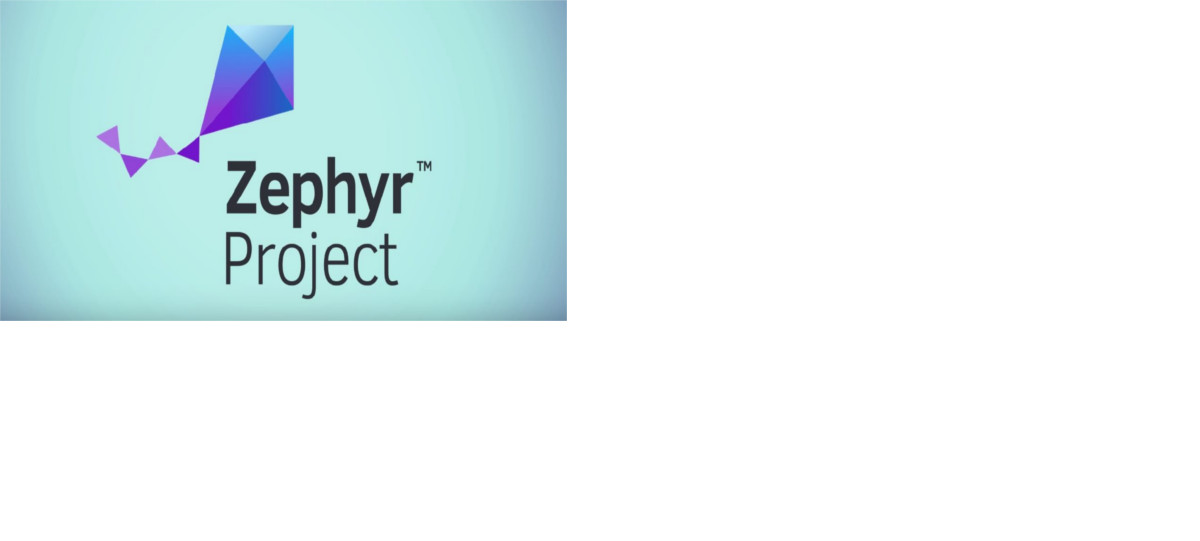
\includegraphics[scale=1.0]{bilder/Zephyr-Project.jpg}			% Titelbild definieren
\end{textblock}

\begin{textblock}{154}(28,135)
	\begin{picture}(150,2)
		\put(0,0){\color{bfhgrey}\rule{150mm}{2mm}}
	\end{picture}
\end{textblock}
\color{black}

% Institution / Titel / Untertitel / Autoren / Experten:
%---------------------------------------------------------------------------
\begin{flushleft}

\vspace*{115mm}

\fontsize{26pt}{28pt}\selectfont 
\titel 				\\							% Titel aus der Datei vorspann/titel.tex lesen
\vspace{2mm}

\fontsize{16pt}{20pt}\selectfont\vspace{0.3em}
Echtzeit-OS f�r das Internet der Dinge 			\\							% Untertitel eingeben
\vspace{5mm}

\fontsize{10pt}{12pt}\selectfont
\textbf{Projektarbeit} \\									% eingeben
\vspace{3mm}

% Abstract (eingeben):
%---------------------------------------------------------------------------
\begin{textblock}{150}(28,190)
\fontsize{10pt}{12pt}\selectfont
Die Linux Foundation hat mit dem Projekt Zephyr mit der Entwicklung eines Echtzeit-Betriebssystems f�r das Internet der Dinge (IoT) begonnen.
Zephyr ist ein Open-Source-Betriebssystem mit dem Ziel ein solides OS f�r IoT Ger�te mit geringen Ressourcen bereitzustellen. Es nutzt eine echtzeitf�hige Kombination aus Nano- und Microkernel. 
Im Gegensatz zu einem Linux Kernel ben�tigt Zephyr nur zwischen 8 und 512 KByte an Arbeitsspeicher.  Aktuell werden folgenden Plattformen unterst�tzt: x86, ARM und ARC EM4
\end{textblock}

\begin{textblock}{150}(28,225)
\fontsize{10pt}{17pt}\selectfont
\begin{tabbing}
xxxxxxxxxxxxxxx\=xxxxxxxxxxxxxxxxxxxxxxxxxxxxxxxxxxxxxxxxxxxxxxx \kill
Studiengang:	\> Elektro- und Kommunikationstechnik			\\
Autoren:		\> Aaron Schmocker, David Wyss					\\
Betreuer:		\> Martin Aebersold								\\
Auftraggeber:	\> Martin Aebersold								\\
Experten:		\> Martin Aebersold								\\
Datum:			\> \versiondate									\\
\end{tabbing}

\end{textblock}
\end{flushleft}

\begin{textblock}{150}(28,280)
\noindent 
\color{bfhgrey}\fontsize{9pt}{10pt}\selectfont
Berner Fachhochschule | Haute �cole sp�cialis�e bernoise | Bern University of Applied Sciences
\color{black}\selectfont
\end{textblock}


\end{titlepage}

%
% ===========================================================================
% EOF
%
                     % activate for Titelseite mit Bild

\cleardoubleemptypage
\setcounter{page}{1}
\cleardoublepage
\phantomsection 
\cleardoubleemptypage
%---------------------------------------------------------------------------

% Table of contents
%---------------------------------------------------------------------------
\tableofcontents
% Versionenkontrolle :
% -----------------------------------------------

\begin{textblock}{180}(15,150)
\color{black}
\begin{huge}
Versionen
\end{huge}
\vspace{10mm}

\fontsize{10pt}{18pt}\selectfont
\begin{tabbing}
xxxxxxxxxxx\=xxxxxxxxxxxxxxx\=xxxxxxxxxxxxxx\=xxxxxxxxxxxxxxxxxxxxxxxxxxxxxxxxxxxxxxxxxxxxxxx \kill
Version	\> Datum	\> Status		\> Bemerkungen \\
0.1	\> 29.09.2016	\> Entwurf		\> Titelblatt erstellt und Template f�r Linux angepasst \\	
%0.2	\> 21.08.2016	\> Entwurf		\> Phasellus scelerisque \\ 
%0.3	\> 02.09.2016	\> Entwurf		\> Donec eget aliquam urna. Lorem ipsum dolor sit amet \\ 
%1.0	\> 12.09.2016	\> Definitiv	\> Lorem ipsum dolor sit ametPhasellus scelerisque, leo sed iaculis ornare \\ 
%1.1	\> 04.11.2016	\> Korrektur	\> Layout angepasst \\
%1.2	\> 01.02.2016	\> Erg�nzung	\> Kapitel 1.1 erweitert \\
\end{tabbing}

\end{textblock}

\cleardoublepage
%---------------------------------------------------------------------------

% Main part:
%---------------------------------------------------------------------------
\pagenumbering{arabic}

% !TeX encoding = ISO-8859-1
\chapter{Management Summary}
\label{chap:managementsummary}

Die Linux Foundation hat mit dem Projekt Zephyr mit der Entwicklung eines
Echtzeit-Betriebssystems f�r das Internet der Dinge (IoT) begonnen.
Zephyr ist ein Open-Source-Betriebssystem mit dem Ziel ein solides OS f�r IoT Ger�te
mit geringen Ressourcen bereitzustellen. Es nutzt eine echtzeitf�hige Kombination aus
Nano- und Microkernel.

Im Gegensatz zu einem Linux Kernel ben�tigt Zephyr nur zwischen 8 und 512 KByte an
Arbeitsspeicher. Aktuell werden folgenden Plattformen unterst�tzt: x86, ARM und ARC
EM4.


\vspace{20mm}
\begin{figure}[h]
	\centering
	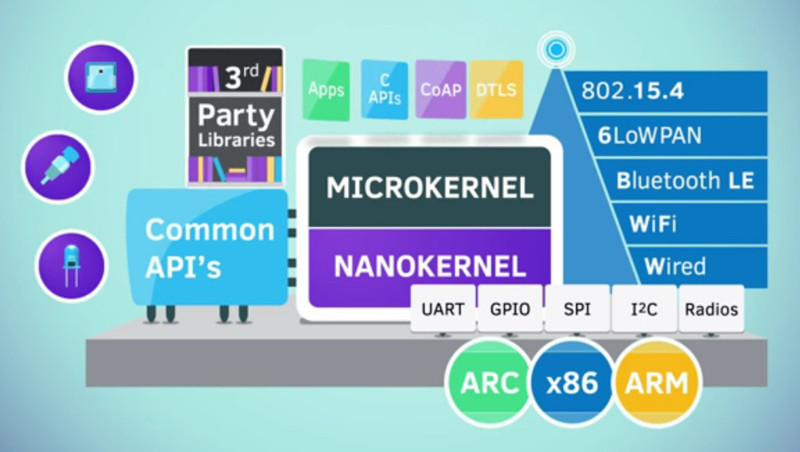
\includegraphics[width=0.7\linewidth]{bilder/zephyr_components.jpg}
	\caption{Komponenten und �bersicht �ber das Zephyr RTOS}
	\label{fig:components}
\end{figure}
\vspace{7mm}

\chapter{Einleitung}
\label{chap:einleitung}

Dieses Dokument dient einerseites zur Illustration der \LaTeX{} Vorlage anhand des Corporate Designs\index{Corporate Design} der Berner Fachhochschule\index{Berner Fachhochschule} und andererseits als Anleitung f�r deren Verwendung. Dabei wird vorausgesetzt, dass der Benutzer bereits Erfahrungen mit \LaTeX{} besitzt oder gewillt ist, sich w�hrend der Benutzung in das Thema einzuarbeiten. Im Quellenverzeichnis sind einige n�tzliche Eintr�ge zu diversen B�chern und Dokumenten im Internet �ber \LaTeX{} zu finden.

% Eintr�ge im Verzeichnis erscheinen lassen ohne hier eine Referenz einzuf�gen
\nocite{kopka:band1}
\nocite{raichle:bibtex_programmierung}
\nocite{MiKTeX}
\nocite{KOMA}
\nocite{TeXnicCenter}
\nocite{Marti06}
\nocite{Erbsland08}
\nocite{juergens:einfuehrung}
\nocite{juergens:fortgeschritten}

\section{Dokumentaufbau}
\label{sec:einleitung_aufbau}

Das vorliegende Dokument ist so aufgebaut wie die Dokumentation einer Projektarbeit oder Thesis\index{Thesis}. Im Kapitel \ref{chap:anleitungen} werden die verwendeten Pakete kurz erkl�rt und Hinweise gegeben, wie die Bibliographie und das Glossar zu verwenden sind. Kapitel \ref{chap:satzspiegeltest} stellt ein reines Beispielkapitel dar, um den Satzspiegel zu pr�fen.

In Abbildung \ref{fig:datei_struktur} ist die Dateistruktur dieses Template dargestellt.

\begin{figure}[H]
	\centering
		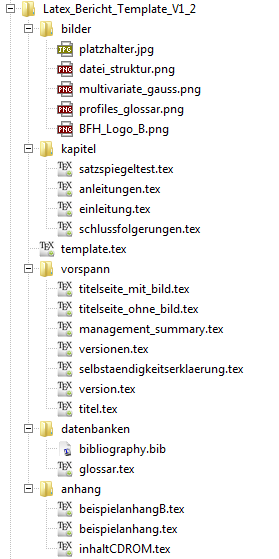
\includegraphics[scale=0.85]{bilder/datei_struktur.png}
	\caption{Dateistruktur}
	\label{fig:datei_struktur}
\end{figure}

\section{Kontakt}
\label{sec:einleitung_kontakt}

Die Hersteller dieser Vorlage sind nat�rlich froh um Verbesserungsvorschl�ge jeder Art. Kapitel \ref{sec:einleitung_vorschlaege} enth�lt m�gliche Verbesserungsvorschl�ge\index{Verbesserungsvorschl�ge}.

\begin{table}[H]
	\centering
		\begin{tabular}{lll} \toprule
			\textbf{Vorname Name} & \textbf{E-Mail} & \textbf{Funktion} \\ \midrule
			Alfred Kaufmann & alfred.kaufmann@bfh.ch & Auftraggeber, Projektleitung, Erg�nzungen \\ \midrule
			Fritz Dellsperger & in Pension & Tipps zur Struktur und Layout \\ \midrule
			David Burri & ausgetreten & Erstellung der Vorlage \\ \bottomrule
		\end{tabular}
	\caption{Kontaktpersonen}
	\label{tab:kontaktpersonen}
\end{table}


\section{Verbesserungsvorschl�ge}
\label{sec:einleitung_vorschlaege}

\begin{itemize}
	\item Erstellen eines eigenen BFH Style-Files
	\item Vorlage f�r die Pr�sentationserstellung mit \LaTeX{}
\end{itemize}



% !TeX encoding = ISO-8859-1
\chapter{Ressourcen, Infrastruktur und Betriebsmittel}
\label{chap:ressourcen}


\section{R�umlichkeiten}

F�r die Arbeit steht ein Arbeitsplatz im Raum T208 zur Verf�gung.

\section{Software und Betriebsysteme}

Da es sich bei Zephyr um ein RTOS handelt, wird die Demoapplikation in C geschrieben. Zur Entwicklung und Dokumentation wird aussschliesslich auf offene Software gesetzt.

\begin{itemize}
	\item Ubuntu 16.04 LT und Arch Linux
	\item Zephyr und Zephyr SDK
	\item GIT
	\item Latex
	\item LibreOffice
\end{itemize}

\section{Hardware}

Folgende Hardware wird f�r das Projekt zur Verf�gung gestellt:

\begin{itemize}
	\item nRF52 Development Kit von Nordic Semiconductor
	\item ST-Link/v2 Debugger
	\item Druck und Temperatur Sensor
	\item Hardware und Computer des Raumes T208:
\end{itemize}

\section{Entwicklungs- und Testwerkzeuge}

\begin{itemize}
	\item Eclipse Neon mit Gnu ARM Plugin
	\item Qt-Creator
	\item SDK und Libraries von Nordic Semiconductors f�r das NRF52 Evalboard
	\item SEGGER J-Link
\end{itemize}

\section{Dokumentation}

Es wird eine Projektdokumentation erwartet, welche die Entwurfsphase sowie die Realisierung und die gemachten
Tests aufzeigt. Alle Dokumente werden auf einem Git-Repository abgelegt. Zur Dokumentation wird auf Latex gesetzt.
\chapter{Definition der Aufgaben}
\label{chap:aufgaben}

\section{Aufgabenbeschreibung}
Im Rahmen der Projektarbeit sollen die Möglichkeiten des Zephyr-OS im Hinblick auf Anwendungen im Bereich \ac{IoT} abgeklärt werden. Besonderer Fokus gilt hierbei dem Vergleich von Zephyr zu bereits bestehenden \ac{RTOS}. Dieser Vergleich soll tabellarisch ersichtlich gemacht werden. Weiter soll im Rahmen der Arbeit eine Demonstratinsapplikation entwickelt werden, auch mit dem Fokus auf das \ac{IoT}.

\section{Anforderungen}

%Folgende Aufgaben sollen im Rahmen der Projektarbeit realisiert werden:

\begin{table}[H]
	\renewcommand{\arraystretch}{1.5}
	\begin{tabular}{|l|}
		\hline
		\textbf{Minimale Anforderung}\\
		\hline
		- Aufsetzen der Entwicklungsumgebung\\
		\hspace{10pt}- Aufsetzen einer Ubuntu-VM\\
		\hspace{10pt}- Einrichten eines Gitrepositories für die Arbeit und Dokumentation\\
		\hspace{10pt}- Inbetriebnahme der GNU ARM Toolchain unter Eclipse Neon\\
		\hspace{10pt}- Installation der SDK und Libraries für das Nordic nRF52-DK\\
		- Evaluation der Fähigkeiten von Zephyr als RTOS für das Internet der Dinge\\
		\hspace{10pt}- Vergleich von Kommunikationsprotokollen mit bestehenden \ac{RTOS}\\
		\hspace{10pt}- Verlgeich der Codebasis mit bestehenden \ac{RTOS}\\
		\hspace{10pt}- Vergleich der Leistungsfähigkeit und Binarygrösse mit bestehenden \ac{ROTS}\\	
		- Entwicklung einer Demonstrationsapplikation\\
		\hspace{10pt}- Mit Fokus auf Anwendungen rund um das Internet der Dinge\\
		\hspace{10pt}- Nutzen von \ac{BLE}\\
		\hspace{10pt}- Nutzen des nRF52-DK\\
		\hline
		\hline
		\textbf{Optionale Erweiterungen}\\
		\hline
		- Portierung des Zephyr-Kernels auf ESP8266\\
		- Entwicklung einer Demoapplikation im Bereich Wireless-Lan\\
		\hline
	\end{tabular}
\end{table}

% !TeX encoding = ISO-8859-1
\chapter{Bedingungen}
\label{chap:bedingungen}

In dieser Projektarbeit sollen die F�higkeiten des Zephyr-ROTS in bestehender Form ausgetestet werden. Spezielle Beachtung soll  den f�r das Internet der Dinge wichtigen Kommunikationsprotokollen wie \ac{BLE} und \ac{NFC} geschenkt werden. Bei der Evaluation und Programmierung der Demoapp sind keine Grenzen gesetzt. 
% !TeX encoding = ISO-8859-1
\chapter{Freigabe}

	\vspace{4em}
	\begin{minipage}{\linewidth}
		\begin{tabular}{p{15em}p{15em}}
			Datum, Unterschrift: &  .......................................................\\
			& \centering Martin Aebersold\\
		\end{tabular}
		\vspace{4em}
	\end{minipage}
	\begin{minipage}{\linewidth}
		\begin{tabular}{p{15em}p{15em}}
			Datum, Unterschrift &  .......................................................\\
			& \centering Aaron Schmocker\\
		\end{tabular}
		\vspace{4em}
	\end{minipage}
	\begin{minipage}{\linewidth}
		\begin{tabular}{p{15em}p{15em}}
			Datum, Unterschrift &  .......................................................\\
			& \centering David Wyss\\
		\end{tabular}
		\vspace{4em}
	\end{minipage}


% Glossary
%---------------------------------------------------------------------------
\phantomsection 
\addcontentsline{toc}{chapter}{Glossar}

\newglossaryentry{BibTeX}{name={BibTeX},description={Programm zur Erstellung von Literaturangaben und -verzeichnissen in \TeX- oder \LaTeX-Dokumenten}}
\newglossaryentry{StwVrz}{name={Stichwortverzeichnis},description={Verzeichnis mit Stichworten aus dem Text}}



%\printglossary
%---------------------------------------------------------------------------
% Bibliography
%---------------------------------------------------------------------------
\phantomsection 
\addcontentsline{toc}{chapter}{Literaturverzeichnis}
%\bibliographystyle{IEEEtranS}
%\bibliography{datenbanken/bibliography}{}
%\printbibliography
%---------------------------------------------------------------------------

%---------------------------------------------------------------------------
\end{document}

